\documentclass[a4paper,12pt]{article}
\usepackage[utf8]{inputenc}
\usepackage[T1]{fontenc}
\usepackage[russian]{babel}
\usepackage{amsmath}
\usepackage{indentfirst}
\usepackage{amsfonts}
\usepackage{amssymb}
\usepackage{makeidx}
\usepackage{graphicx}
\usepackage{fancyhdr}
\usepackage{dsfont}
\usepackage{cancel}
\usepackage{textcomp}
\usepackage{setspace} 
\usepackage{pdfpages}
\usepackage{nccmath}
\usepackage[left=2cm,right=2cm,top=2cm,bottom=2cm,bindingoffset=0cm]{geometry}
\usepackage[linesnumbered,boxed]{algorithm2e}
\graphicspath{{./images/}}
\onehalfspacing 
\pagestyle{fancy}
\fancyhf{}
\fancyhead[RE,LO]{Курсовая работа: Мусатов Д.Ю } 
\fancyhead[LE,RO]{Сеточные модели уравнений с ЧП} 
\fancyfoot[RE,LO]{\leftmark} 
\fancyfoot[LE,RO]{\thepage}  
\renewcommand{\headrulewidth}{2pt} 
\renewcommand{\footrulewidth}{1pt} 
\usepackage{titlesec}
\usepackage{xcolor}
\usepackage{hyperref} 
\usepackage{tabularx}
\usepackage{amsmath,amssymb,amsthm}
\newcolumntype{C}{>{\centering\arraybackslash}X}
\definecolor{linkcolor}{HTML}{000000}
\definecolor{urlcolor}{HTML}{799B03}
\titleformat{\section}[block]{\Large\bfseries\filcenter}{\thesection}{1em}{}
\hypersetup{pdfstartview=FitH, linkcolor=linkcolor,urlcolor=urlcolor, colorlinks=true}

\usepackage{listings}
\lstset{ %
	language=Python,                 % выбор языка для подсветки (здесь это С)
	basicstyle=\small\sffamily, % размер и начертание шрифта для подсветки кода
	numbers=left,               % где поставить нумерацию строк (слева\справа)
	numberstyle=\tiny,           % размер шрифта для номеров строк
	stepnumber=1,                   % размер шага между двумя номерами строк
	numbersep=5pt,                % как далеко отстоят номера строк от подсвечиваемого кода
	backgroundcolor=\color{white}, % цвет фона подсветки - используем \usepackage{color}
	showspaces=false,            % показывать или нет пробелы специальными отступами
	showstringspaces=false,      % показывать или нет пробелы в строках
	showtabs=false,             % показывать или нет табуляцию в строках
	frame=single,              % рисовать рамку вокруг кода
	tabsize=2,                 % размер табуляции по умолчанию равен 2 пробелам
	captionpos=t,              % позиция заголовка вверху [t] или внизу [b] ё
	breaklines=true,           % автоматически переносить строки (да\нет)
	breakatwhitespace=false, % переносить строки только если есть пробел
	escapeinside={\%*}{*)},   % если нужно добавить комментарии в коде
	inputencoding=utf8,
	extendedchars=false,
}
\begin{document}
	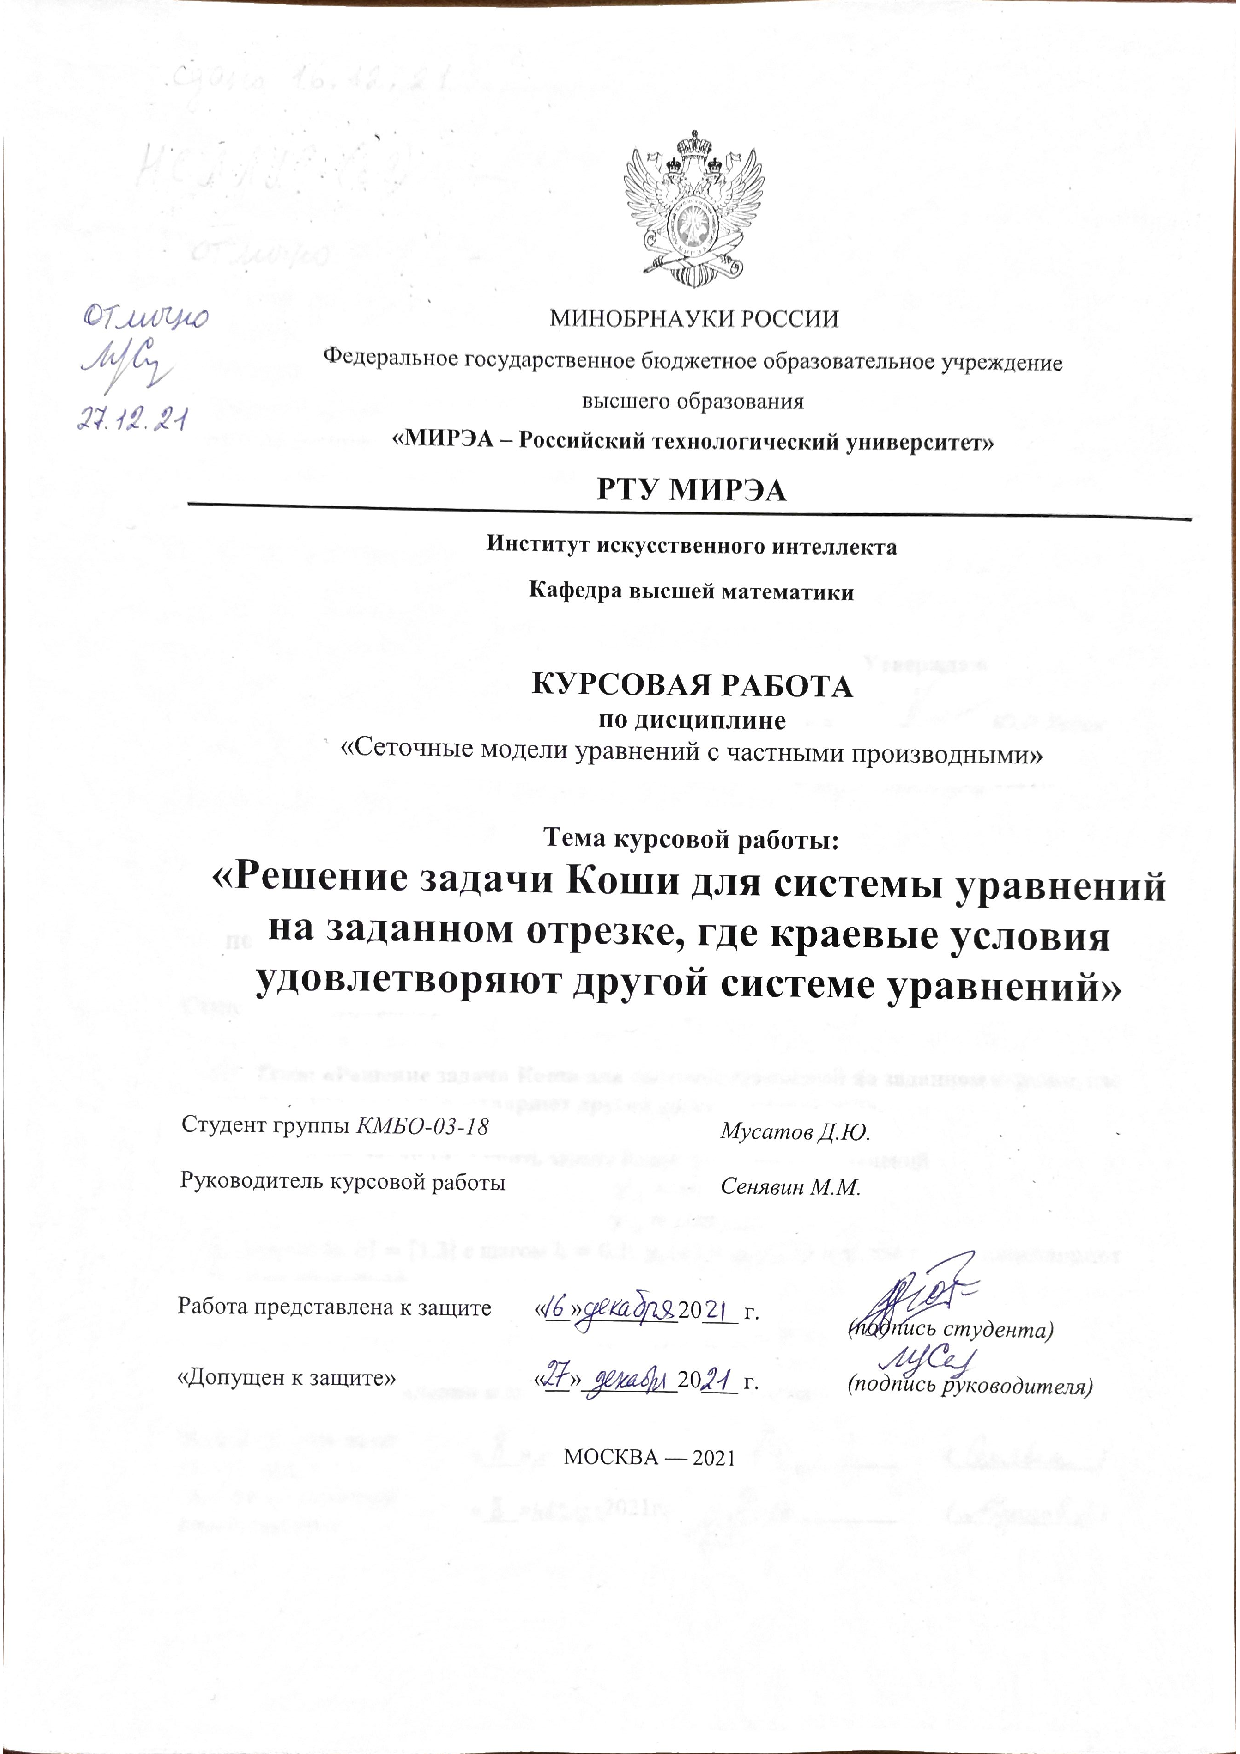
\includepdf[pages=-]{titul}
	\setcounter{section}{0}
	\setcounter{page}{2}
	\tableofcontents
	\clearpage
	\section{Введение. Постановка задачи}
	\textbf{Вариант №15}
	
	Необходимо решить задачу коши для системы уравнений:
$$
\begin{array}{c}
	y'_{1}=sin(y_{2})\\
	y'_{2}=cos(y_{1})	
\end{array}
$$
на отрезке $ [a,b]=[1,3] $ с шагом $ h=0.1;\;\; y_{1}(a)=p,\;\;y_{2}(a)=q,$ где $ p $ и $ q $ удовлетворяют системе уравнений:
$$
\begin{array}{c}
	p^{2}+q^{2}=1\\
	sin(p-q)+0.3p=1
\end{array}
$$

Разобъём поставленную задачу на два этапа:
\begin{enumerate}
	\item Нахождение $ p $ и $ q $, удовлетворяющих системе уравнений
	$$
	\begin{array}{c}
		p^{2}+q^{2}=1\\
		sin(p-q)+0.3p=1
	\end{array}
	$$
	\item Решение задачи Коши для системы уравнений
	$$
	\begin{array}{c}
		y'_{1}=sin(y_{2})\\
		y'_{2}=cos(y_{1})	
	\end{array}
	$$
	на отрезке $ [a,b]=[1,3] $ с шагом $ h=0.1;$ и начальными условиями $ y_{1}(a)=p,\;y_{2}(a)=q$
\end{enumerate}

Решение этапов будем проводить последовательно: найдем p и q (первый этап - решение нелинейной системы алгебраических уравнений (НСЛАУ)), затем будем использовать этот результат как входную информацию для решения задачи Коши для системы уравнений (второй этап - решение системы обыкновенных дифференцциальных уравнений (СДУ)).
\clearpage
\section{Теоретический обзор}

\subsection{Решение нелинейных уравнений}

Рассмотрим уравнение вида: $f(x)=0$, где $f(x)-$ функция, определенная и непрерывная на некотором промежутке. Требуется найти корни данного уравнения. Оно ищется в два этапа:

1. Находятся отрезки $\left[a_{i}, b_{i}\right]$, внутри каждого из которых содержится ровно один корень.

2. С помощью того или иного итерационного метода значения корней уточняются.

Одним из итерационных методов вычисления корней является метод Ньютона.

\subsection{Метод Ньютона (метод касательных)}

Метод Ньютона или касательных заключается в том, что если $x_{n}-$ некоторое приближение к корню $x_{*}$ уравнения $f(x)=0, f \in C^{1}$, то следующее приближение определяется как корень касательной к функции $f(x)$, проведенной в точке $x_{n}$.

Уравнение касательной к функции $f(x)$ в точке $x_{n}$ имеет вид:

$$
f^{\prime}\left(x_{j}\right)=\frac{y-f\left(x_{n}\right)}{x-x_{n}}
$$

В уравнении касательной положим $y=0$ и $x=x_{n+1}$.

Тогда алгоритм последовательных вычислений в методе Ньютона состоит в следующем:

$$
x_{n+1}=x_{n}-\frac{f\left(x_{n}\right)}{f^{\prime}\left(x_{n}\right)}
$$

Сходимость метода касательных квадратичная, порядок сходимости равен $2 .$

Таким образом, метод Ньютона (метод касательных) применяется в том случае, если уравнение $f(x)=0$ имеет корень $x \in[a ; b]$, и выполняются условия:

1) функция $y=f(x)$ определена и непрерывна при $x \in[a ; b]$;

2) $f(a) \cdot f(b)<0$ (функция принимает значения разных знаков на концах отрезка $[a ; b])$;

3) производные $f(x)$ и $f^{\prime}(x)$ сохраняют знак на отрезке $[a ; b]$ (т.е. функция $f(x)$ либо возрастает, либо убывает на отрезке $[a ; b]$, сохраняя при этом направление выпуклости);

4) $f^{\prime}(x) \neq 0$ при $x \in[a ; b]$.

Геометрически этот метод означает замену на каждой итерации графика $y=$ $f(x)$ касательной к нему. Для метода Ньютона имеет место следующая оценка:

$$
\left|x_{n}-x^{*}\right| \leq \frac{M_{2}}{2 m_{1}} \cdot\left|x_{n}-x_{n-1}\right|^{2}, \text { где } M_{2}=\max _{a \leq x b}\left|f^{\prime \prime}(x)\right|, m_{1}=\min _{a \leq x b}\left|f^{\prime}(x)\right| .
$$

\subsection{Решение систем нелинейных уравнений}

Систему нелинейных уравнений можно записать в координатном виде

$$
f_{k}\left(x_{1}, x_{2}, x_{3}, \ldots, x_{n}\right)=0,1 \ll k \ll n .
$$

Такие системы решаются практически только итерационными методами. Нулевое приближение в случае двух переменных можно найти графически: построить на плоскости $\left(x_{1}, x_{2}\right)$ кривые $f_{1}\left(x_{1}, x_{2}\right)=0$ и $f_{2}\left(x_{1}, x_{2}\right)=0$ и найти точки их пересечения.

\subsection{Метод Ньютона для решения системы нелинейных уравнений}

Пусть известно некоторое приближение $x^{(s)}$ к корню $\bar{x} .$ Как и для одной переменной, запишем исходную систему в виде $f\left(x^{(s)}+\Delta x\right)=0$, где $\Delta x=\bar{x}-x^{(s)}$. Разлагая эти уравнения в ряды и ограничиваясь первыми дифференциалами, т.е. линеаризуя функцию, получим

$$
\sum_{i=1}^{n} \frac{\partial f_{k}\left(x^{(s)}\right)}{\partial x_{i}} \Delta x_{i}^{(s)}=-f_{k}\left(x^{(s)}\right), 1 \leq k \leq n .
$$

Эта система уравнений, линейных относительно приращений $\Delta x_{i}^{(s)}$, все коэффициенты этой системы выражаются через последнее приближение $x^{(s)}$. Решив эту систему, найдем новое приближение $x^{(s+1)}=x^{(s)}+\Delta x^{(s)}$.

Метод Ньютона можно свести к методу последовательных приближений, положив $\varphi(x)=x-\left[\frac{\partial f}{\partial x}\right]^{-1} f(x)$, где $\left[\frac{\partial f}{\partial x}\right]^{-1}$ есть матрица, обратная матрице производных.

Аналогично проводится теоретический анализ условий сходимости. Если нулевое приближение выбрано удачно, то метод Ньютона сходится, причем очень быстро. Поэтому на практике этот метод используют чаще всего.

В отличие от других методов решения систем нелинейных уравнений, для метода Ньютона хорошим критерием окончания итераций является условие $\left\|x^{(s)}-x^{(s+1)}\right\| \leq \varepsilon .$ В самом деле, вблизи корня ньютоновские итерации сходятся квадратично, поэтому если этот критерий выполнен, то $\left\|x^{(s+1)}-\bar{x}\right\| \approx \varepsilon^{2} \leq \varepsilon$.

Сходимость итераций исследуем так же, как и для одной переменной. Обозначим компоненты решения через $\bar{x}_{k}$ и преобразуем погрешность очередной итерации 

$$
\begin{aligned}
	x_{k}^{(s+1)}-\overline{x_{k}}=f_{k}\left(x_{1}^{(s)}, \ldots, x_{n}^{(s)}\right)-f_{k}\left(\overline{x_{1}}, \ldots, \overline{x_{n}}\right)=f_{k}\left(x^{(s)}\right)&-f_{k}(\overline{\mathrm{x}}) =\left[\frac{\partial f_{k}\left(\xi_{k}\right)}{\partial l}\right] \rho\left(x^{(s)}, \overline{\mathrm{x}}\right) \\
	&=\sum_{i=1}^{n}\left(x_{i}^{(s)}-\bar{x}_{l}\right)\left[\frac{\partial f_{k}\left(\xi_{k}\right)}{\partial x_{i}}\right],
\end{aligned}
$$

где $l$ - направление, соединяющее многомерные точки $x^{(s)}$ и $\bar{x}$, а $\xi_{k}-$ некоторая точка, лежащая между ними на этом направлении. Это равенство означает, что вектор погрешности нового приближения равен матрице производных, умноженной на вектор погрешности предыдущего приближения.

\subsection{Задача Коши}

Обыкновенное дифференциальное уравнение р-го порядка

$$
u^{(p)}(x)=f\left(x, u, u^{\prime}, u^{\prime \prime}, \ldots, u^{(p-1)}\right)
$$

при помощи замены $u^{(k)}(x) \equiv u_{k}(x)$ можно свести к эквивалентной системе р уравнений первого порядка

$$
\begin{gathered}
	u_{k}^{\prime}(x)=u_{k+1}(x), 0 \leq k \leq p-2, \\
	u_{p-1}^{\prime}(x)=f\left(x, u_{0}, u_{1}, \ldots, u_{p-1}\right)
\end{gathered}
$$

где $u_{0}(x) \equiv u(x) .$ Аналогично, произвольную систему дифференциальных уравнений любого порядка можно заменить некоторой эквивалентной системой уравнений первого порядка

$$
u_{k}^{\prime}(x)=f_{k}\left(x, u_{1}, u_{2}, \ldots, u_{p}\right), \quad 1 \leq k \leq p
$$

Система р-го порядка имеет множество решений, которое в общем случае зависит от $\mathrm{p}$ параметров $c=\left\{c_{1}, c_{2}, \ldots, c_{p}\right\}$. Для определения значений этих параметров, т.е. для выделения единственного (или нужного) решения, надо наложить р дополнительных условий на функции $u_{k}(x)$.

Задача Коши (задача с начальными условиями) имеет дополнительные условия вида $u_{k}(\xi)=\eta_{k^{\prime}} 1 \leq k \leq p$, т.е. заданы значения всех функций в одной и той же точке $x=\xi .$ Эти условия можно рассматривать как задание координат начальной точки $\left(\xi, \eta_{1}, \eta_{2}, \ldots, \eta_{p}\right)$ интегральной кривой в $(\mathrm{p}+1)$-мерном пространстве $\left(x, u_{1}, u_{2}, \ldots, u_{p}\right) .$ Решение при этом требуется найти на некотором отрезке $\xi \leq x \leq X$, так что точку $\mathrm{x}=\xi$ можно считать начальной точкой этого отрезка.

\subsection{Метод Эйлера}
 Простейший численный метод решения систем обыкновенных дифференциальных уравнений.
 Пусть дана задача Коши для уравнения первого порядка:
 
$$\begin{aligned}
 \dfrac{dy}{dx}=f(x,y),\\
 y_{{|_{{x=x_{0}}}}}=y_{0},\end{aligned} $$
 
 где функция f определена на некоторой области  $ D\subset \mathbb{R} ^{2} $. Решение ищется на интервале $ (x_{0},b] $. На этом интервале введем узлы: $ x_{0}<x_{1}<\dots <x_{n}\leq b $. Приближенное решение в узлах $ x_{i} $, которое обозначим через $ y_{i} $, определяется по формуле:
 $$ y_{i}=y_{{i-1}}+(x_{i}-x_{{i-1}})f(x_{{i-1}},y_{{i-1}}),\quad i=1,2,3,\dots ,n. $$
 
 Эти формулы непосредственно обобщаются на случай систем обыкновенных дифференциальных уравнений.

\subsection{Метод Рунге-Кутты}

Метод, позволяющий строить схемы различного порядка точности. Наиболее используемы схемы четвертого порядка точности, образующие семейство четырехчленных схем. Метод Рунге- Кутты четвёртого порядка при вычислениях с постоянным шагом интегрирования столь широко распространён, что его часто называют просто методом Рунге — Кутты.

Рассмотрим задачу Коши для системы обыкновенных дифференциальных уравнений первого порядка

$$
y^{\prime}=f(x, y), \quad y\left(x_{0}\right)=y_{0} .
$$

Тогда приближенное значение в последующих точках вычисляется по итерационной формуле:

$$
y_{n+1}=y_{n}+\frac{h}{6}\left(K_{1}+2 K_{2}+2 K_{3}+K_{4}\right)
$$

Вычисление нового значения проходит в четыре стадии:

$$
\begin{gathered}
	K_{1}=f\left(x_{n}, y_{n}\right), \\
	K_{2}=f\left(x_{n}+\frac{h}{2}, y_{n}+\frac{h}{2} K_{1}\right), \\
	K_{3}=f\left(x_{n}+\frac{h}{2}, y_{n}+\frac{h}{2} K_{2}\right), \\
	K_{4}=f\left(x_{n}+h, y_{n}+h K_{3}\right),
\end{gathered}
$$

где $\mathrm{h}$ - величина шага сетки по $\mathrm{x}$. Этот метод имеет четвёртый порядок точности. Это значит, что ошибка на одном шаге имеет порядок $O\left(h^{5}\right)$, а суммарная ошибка на конечном интервале интегрирования имеет порядок $O\left(h^{4}\right)$.

На случай систем уравнений схему Рунге-Кутты легко переносятся, как во всех других методах, при помощи формальной замены у, $f(x, y)$ на $\boldsymbol{y}, f(x, \boldsymbol{y})$. Например, для системы двух уравнений

$$
\begin{aligned}
	&u^{\prime}(x)=f(x, u(x), v(x)), \\
	&v^{\prime}(x)=q(x, u(x), v(x)),
\end{aligned}
$$

обозначая через у, $\mathrm{z}$ приближенные значения функций $u(x), v(x)$, запишем аналогичную четырехчленную схему следующим образом:

$$
\begin{aligned}
	&y_{n+1}=y_{n}+\frac{h}{6}\left(K_{1}+2 K_{2}+2 K_{3}+K_{4}\right), \\
	&z_{n+1}=z_{n}+\frac{h}{6}\left(Q_{1}+2 Q_{2}+2 Q_{3}+Q_{4}\right),
\end{aligned}
$$

где

$$
\begin{gathered}
	K_{1}=f\left(x_{n}, y_{n}, z_{n}\right), \\
	Q_{1}=q\left(x_{n}, y_{n}, z_{n}\right), \\
	K_{2}=f\left(x_{n}+\frac{h}{2}, y_{n}+\frac{h}{2} K_{1}, z_{n}+\frac{h}{2} Q_{1}\right),
\end{gathered}
$$



$$
\begin{aligned}
	&Q_{2}=q\left(x_{n}+\frac{h}{2}, y_{n}+\frac{h}{2} K_{1}, z_{n}+\frac{h}{2} Q_{1}\right) \\
	&K_{3}=f\left(x_{n}+\frac{h}{2}, y_{n}+\frac{h}{2} K_{2}, z_{n}+\frac{h}{2} Q_{2}\right) \\
	&Q_{3}=q\left(x_{n}+\frac{h}{2}, y_{n}+\frac{h}{2} K_{2}, z_{n}+\frac{h}{2} Q_{2}\right) \\
	&K_{4}=f\bigg(x_{n}+h, y_{n}+h K_{3}, z_{n}+h Q_{3}\bigg) \\
	&Q_{4}=q\bigg(x_{n}+h, y_{n}+h K_{3}, z_{n}+h Q_{3}\bigg)
\end{aligned}
$$
\clearpage
\section{Решение поставленной задачи}
\subsection{1 этап - Решение НСЛАУ}
Найдём значения p и q, удовлетворяющие системе уравнений:
$$
\begin{array}{c}
	p^{2}+q^{2}=1\\
	sin(p-q)+0.3p=1
\end{array}
$$
Построим график. Воспользуемся для построения онлайн калькулятором Desmos. Получим следующее изображение:

\begin{center}
	\includegraphics[scale=1]{1}\\
	\color{blue}
	Рисунок 1. график функций принадлежащих системе
\end{center}

Как видно из графика, есть два пересечения функций — существует два решения данной системы нелинейных уравнений.

\begin{center}
	\textbf{Метод Ньютона для решения системы нелинейных уравнений:}
\end{center}
Рассмотрим сначала точку пересечения в первой четверти. По графику определим начальное приближение $ x_{0}=(1,0) $. Найдем его решениe с помощью метода Ньютона.

Найдем матрицу Якоби $ w $, это матрица частных производных каждого уравнения. Определитель матрицы Якоби для $ x_{0} $ должен быть не равен 0.

Найдем вектор приращений, который рассчитывается как 
$dx = -w^{-1} \cdot f(x_{0}) $. Найдем вектор решения $ x=x_{0}+ dx $. Проверяем условие сходимости: разность $ x-x_{0} $ должна быть меньше точности вычислений.

 Зададим точность вычислений: $e  = 0.00001 $.
 \renewcommand{\arraystretch}{2}
\begin{center}
	
\begin{table}[htbp]\scriptsize
	\begin{tabularx}{\textwidth}{|>{\hsize=0.12\hsize}C|>{\hsize=0.19\hsize}C|>{\hsize=0.1\hsize}C|>{\hsize=0.1\hsize}C|>{\hsize=0.1\hsize}C|>{\hsize=0.11\hsize}C|>{\hsize=0.2\hsize}C|}
		\hline
	Итерация & Матрица Якоби w & p & q & $ f_1(p,q) $ &$ f_2(p,q) $& $max(p-p_{0},q-q_{0})  $\\
	\hline
	1 & $ \bigg[\begin{smallmatrix}
		2 & 0 \\
		0.840302 & -0.540302
	\end{smallmatrix}\bigg] $ & 1 & 0.261837 & 0.0685585 & -0.0270695	& 0.261837 \\
\hline
	2 & $ \bigg[\begin{smallmatrix}
			2 & 0.523673 \\
			1.03971 & -0.739706
		\end{smallmatrix}\bigg] $ & 0.981947  & 0.199867  &   0.00416625 & -0.00065927	& 0.06197\\
		\hline
	3 & $ \bigg[\begin{smallmatrix}
		 1.96389 & 0.399733 \\
		1.00945 & -0.709449
	\end{smallmatrix}\bigg] $ &  0.980448   &  0.196806  &  0.0000115 &  -0.00000084 	& 0.00306121\\
	\hline
	4 & $ \bigg[\begin{smallmatrix}
	1.9609 & 0.393611 \\
	1.00835 & -0.708347
	\end{smallmatrix}\bigg] $ &  0.980444 & 0.196798 &  0 & -0.00000008	& 0.00000745\\
	\hline
	\end{tabularx}
\end{table}
\color{blue}
Таблица 1. результаты вычислений методом Ньютона начальное приближение (1,0)
\end{center}
 Ответ: p = 0.980444, q = 0.196798;\\
 
 Рассмотрим точку пересечения функций в третьей четверти. По графику определим начальное приближение $ x_{0}=(0,-1) $.
 
 Методом Ньютона получим следующее решение:
 \begin{center}
	\renewcommand{\arraystretch}{2}

\begin{table}[htbp]\scriptsize
	\begin{tabularx}{\textwidth}{|>{\hsize=0.12\hsize}C|>{\hsize=0.19\hsize}C|>{\hsize=0.1\hsize}C|>{\hsize=0.1\hsize}C|>{\hsize=0.1\hsize}C|>{\hsize=0.11\hsize}C|>{\hsize=0.2\hsize}C|}
		\hline
	Итерация & Матрица Якоби w & p & q & $ f_1(p,q) $ &$ f_2(p,q) $& $max(p-p_{0},q-q_{0})  $\\
	\hline
	1 & $ \bigg[\begin{smallmatrix}
		0 & -2 \\
		0.804302 & -0.540302
	\end{smallmatrix}\bigg] $ & 0.188657 & -1 & 0.0355915 & -0.0155338	& 0.188657 \\
\hline
	2 & $ \bigg[\begin{smallmatrix}
			0.377314 & -2 \\
			0.672906 & -0.372906
		\end{smallmatrix}\bigg] $ & 0.22545 &  -0.975263 &  0.00196564 & -0.0000676	& 0.0367932\\
		\hline
	3 & $ \bigg[\begin{smallmatrix}
		 0.450901 & -1.95053 \\
		0.661693 & -0.361693
	\end{smallmatrix}\bigg] $ &  0.226198  &  -0.974081 &  0.0000019 &  -0.00000006 	& 0.00118059\\
	\hline
	4 & $ \bigg[\begin{smallmatrix}
	0.452396 & -1.94816 \\
	0.662097 & -0.362097
	\end{smallmatrix}\bigg] $ &  0.226199 & -0.974081 &  0 & -0.00000002	& 0.00000113\\
	\hline
	\end{tabularx}
\end{table}
\color{blue}
Таблица 2. результаты вычислений методом Ньютона начальное приближение (0,-1)
\end{center}
 Ответ: p = 0.226199, q = -0.974081;\\
 
 Выполним проверку с помощью онлайн калькуляторов, позволяющих решить НСЛАУ
\begin{center}
	 \includegraphics[scale=1]{2}\\
	 \color{blue}
	 Рисунок 2. Результат решения системы с помощью онлайн калькуляторов
\end{center}
Как можем видеть, результаты совпали с точностью до $ 10^{-5} $. Проверку выполнили. Код программы представлен в приложении.
\clearpage
\subsection{2 этап - Решение СДУ}
Найдем решение задачи Коши для системы уравнений:
$$
\begin{array}{c}
	y'_{1}=sin(y_{2})\\
	y'_{2}=cos(y_{1})	
\end{array}
$$
на отрезке $ [a,b]=[1,3] $ с шагом $ h=0.1;\;\;$

На первом этапе, в ходе вычислений, получили два решения системы.
$$
\begin{array}{c}
	p_{1} = 0.980444, q_{1} = 0.196798;\\
	p_{2} = 0.226199, q_{2} = -0.974081;
\end{array}
$$

Значит, краевые условия следующие, обозначим с помощью верхних индексов номера решений:
$$
\begin{array}{c}
	y^{1}_{1}(1) = 0.980444,\quad y^{1}_{2}(1) = 0.196798;\\
	y^{2}_{1}(1)  = 0.226199, \quad y^{2}_{2}(1) = -0.974081;
\end{array}
$$  
Будем искать решение, используя методы Эйлера и Рунге-Кутта 4-го порядка.

Использую решение методом Рунге-Кутты получим следующий график и таблицу:
\begin{center}
	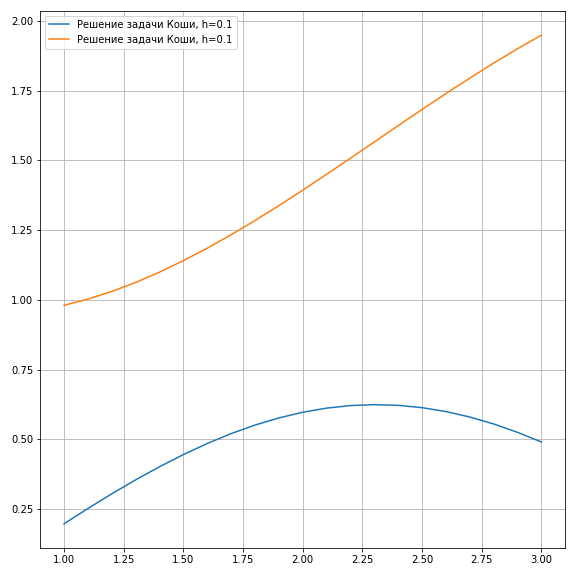
\includegraphics[scale=0.49]{plot_1}\\
	\color{blue}
	Рисунок 3. Графики функций СДУ с краевыми условиями 	$ y^{rq1}_{1},  y^{rq1}_{2} $
\end{center}

\renewcommand{\arraystretch}{1.284}
\begin{center}
	\begin{table}[htbp]
		\footnotesize
		\begin{tabular}{|c|c|c|c|c|c|c|c|c|c|}
			\hline
			$ y_{1} $ & $ k_{1} $ & $ k_{2} $ & $ k_{3} $ & $ k_{4} $ & $ y_{2} $ & $ q_{1} $ & $ q_{2} $ & $ q_{3} $ & $ q_{4} $ \\
			\hline
			0.98044 & 0.01955 & 0.02227 & 0.02223 & 0.02489 & 0.1968 & 0.05567 & 0.05485 & 0.05474 & 0.0538 \\
			\hline
			1.00269 & 0.02489 & 0.02749 & 0.02744 & 0.02995 & 0.25157 & 0.0538 & 0.05275 & 0.05264 & 0.05147 \\
			\hline
			1.03014 & 0.02996 & 0.0324 & 0.03234 & 0.0347 & 0.30425 & 0.05147 & 0.05018 & 0.05007 & 0.04867 \\
			\hline
			1.06249 & 0.0347 & 0.03697 & 0.0369 & 0.03907 & 0.35436 & 0.04867 & 0.04715 & 0.04705 & 0.04541 \\
			\hline
			1.09941 & 0.03907 & 0.04115 & 0.04107 & 0.04305 & 0.40143 & 0.04541 & 0.04366 & 0.04357 & 0.04172 \\
			\hline
			1.14051 & 0.04305 & 0.04492 & 0.04483 & 0.04659 & 0.44503 & 0.04171 & 0.03975 & 0.03966 & 0.0376 \\
			\hline
			1.18537 & 0.0466 & 0.04825 & 0.04816 & 0.04969 & 0.48472 & 0.0376 & 0.03543 & 0.03535 & 0.03309 \\
			\hline
			1.23355 & 0.0497 & 0.05113 & 0.05102 & 0.05233 & 0.52009 & 0.03309 & 0.03073 & 0.03067 & 0.02823 \\
			\hline
			1.28461 & 0.05234 & 0.05353 & 0.05343 & 0.0545 & 0.55078 & 0.02823 & 0.02571 & 0.02565 & 0.02307 \\
			\hline
			1.33807 & 0.05451 & 0.05547 & 0.05536 & 0.0562 & 0.57645 & 0.02306 & 0.0204 & 0.02036 & 0.01764 \\
			\hline
			1.39346 & 0.0562 & 0.05693 & 0.05682 & 0.05742 & 0.59682 & 0.01764 & 0.01487 & 0.01483 & 0.01202 \\
			\hline
			1.45031 & 0.05742 & 0.05791 & 0.0578 & 0.05817 & 0.61167 & 0.01202 & 0.00916 & 0.00914 & 0.00626 \\
			\hline
			1.50815 & 0.05817 & 0.05842 & 0.05831 & 0.05844 & 0.62082 & 0.00626 & 0.00336 & 0.00334 & 0.00043 \\
			\hline
			1.56649 & 0.05844 & 0.05846 & 0.05834 & 0.05824 & 0.62416 & 0.00043 & -0.00249 & -0.00249 & -0.0054 \\
			\hline
			1.62487 & 0.05824 & 0.05802 & 0.0579 & 0.05756 & 0.62167 & -0.00541 & -0.00831 & -0.0083 & -0.01117 \\
			\hline
			1.68281 & 0.05756 & 0.05711 & 0.05699 & 0.05641 & 0.61338 & -0.01118 & -0.01403 & -0.01401 & -0.01682 \\
			\hline
			1.73984 & 0.05641 & 0.05571 & 0.0556 & 0.05479 & 0.59936 & -0.01682 & -0.0196 & -0.01956 & -0.02228 \\
			\hline
			1.79548 & 0.05478 & 0.05385 & 0.05374 & 0.05269 & 0.57979 & -0.02228 & -0.02494 & -0.0249 & -0.02748 \\
			\hline
			1.84925 & 0.05268 & 0.05151 & 0.0514 & 0.05012 & 0.55488 & -0.02749 & -0.03001 & -0.02995 & -0.03239 \\
			\hline
			1.90069 & 0.05011 & 0.04871 & 0.0486 & 0.04708 & 0.52492 & -0.03239 & -0.03475 & -0.03469 & -0.03695 \\
			\hline
			1.94933 & & & & & 0.49021 &  & & &  \\
			\hline
	\end{tabular}\\
\end{table}
\color{blue}
Таблица №3. таблица коэффициентов для метода Рунге-Кутты на кажоый итерации для краевых условий $ y^{rq1}_{1}, \; y^{rq1}_{2} $ 
\end{center}

\begin{center}
	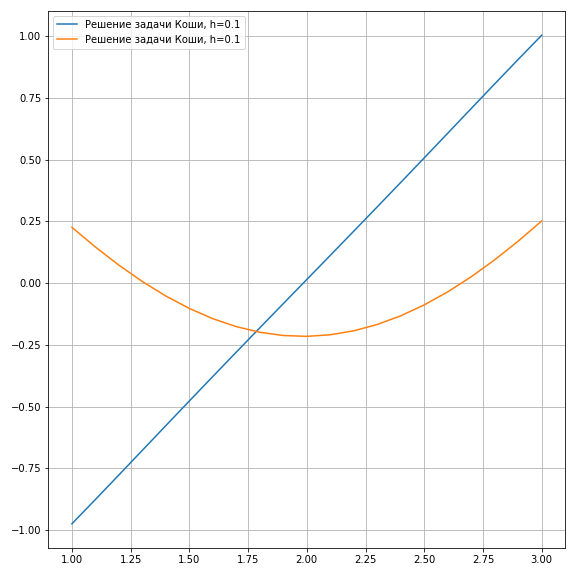
\includegraphics[scale=0.49]{plot_2}\\
	\color{blue}
	Рисунок 4. Графики функций СДУ с краевыми условиями 	$ y^{rq2}_{1},  y^{rq2}_{2} $
\end{center}
\clearpage

\renewcommand{\arraystretch}{1.284}
\begin{center}
\begin{table}[htbp]
	\footnotesize
		\begin{tabular}{|c|c|c|c|c|c|c|c|c|c|}
			\hline
			$ y_{1} $ & $ k_{1} $ & $ k_{2} $ & $ k_{3} $ & $ k_{4} $ & $ y_{2} $ & $ q_{1} $ & $ q_{2} $ & $ q_{3} $ & $ q_{4} $ \\
			\hline
			0.2262 & -0.08272 & -0.07988 & -0.07986 & -0.07681 & -0.97408 & 0.09745 & 0.0983 & 0.09827 & 0.09893 \\
			\hline
			0.14637 & -0.07681 & -0.07355 & -0.07353 & -0.07007 & -0.87583 & 0.09893 & 0.09942 & 0.0994 & 0.09973 \\
			\hline
			0.07286 & -0.07007 & -0.06643 & -0.06642 & -0.06261 & -0.77644 & 0.09973 & 0.09993 & 0.09992 & 0.1 \\
			\hline
			0.00646 & -0.06261 & -0.05863 & -0.05864 & -0.05451 & -0.67654 & 0.1 & 0.09997 & 0.09997 & 0.09986 \\
			\hline
			-0.05215 & -0.05452 & -0.05026 & -0.05027 & -0.0459 & -0.57658 & 0.09986 & 0.09968 & 0.0997 & 0.09948 \\
			\hline
			-0.1024 & -0.0459 & -0.04143 & -0.04144 & -0.03687 & -0.47689 & 0.09948 & 0.09922 & 0.09924 & 0.09897 \\
			\hline
			-0.14382 & -0.03688 & -0.03223 & -0.03225 & -0.02753 & -0.37767 & 0.09897 & 0.09869 & 0.09872 & 0.09845 \\
			\hline
			-0.17604 & -0.02754 & -0.02277 & -0.02278 & -0.01797 & -0.27896 & 0.09845 & 0.0982 & 0.09825 & 0.09803 \\
			\hline
			-0.19882 & -0.01797 & -0.01313 & -0.01314 & -0.00827 & -0.18073 & 0.09803 & 0.09785 & 0.0979 & 0.09776 \\
			\hline
			-0.21195 & -0.00828 & -0.0034 & -0.0034 & 0.00149 & -0.08285 & 0.09776 & 0.09767 & 0.09773 & 0.09769 \\
			\hline
			-0.21535 & 0.00149 & 0.00637 & 0.00637 & 0.01124 & 0.01486 & 0.09769 & 0.09771 & 0.09776 & 0.09782 \\
			\hline
			-0.20898 & 0.01124 & 0.01608 & 0.01609 & 0.0209 & 0.1126 & 0.09782 & 0.09794 & 0.09799 & 0.09815 \\
			\hline
			-0.1929 & 0.0209 & 0.02567 & 0.02568 & 0.03041 & 0.21057 & 0.09815 & 0.09834 & 0.09838 & 0.09861 \\
			\hline
			-0.16723 & 0.0304 & 0.03506 & 0.03507 & 0.03966 & 0.30894 & 0.0986 & 0.09885 & 0.09888 & 0.09913 \\
			\hline
			-0.13217 & 0.03966 & 0.04416 & 0.04417 & 0.04857 & 0.4078 & 0.09913 & 0.09937 & 0.09939 & 0.09961 \\
			\hline
			-0.08803 & 0.04857 & 0.05286 & 0.05287 & 0.05704 & 0.50718 & 0.09961 & 0.0998 & 0.09981 & 0.09994 \\
			\hline
			-0.03518 & 0.05704 & 0.06107 & 0.06107 & 0.06495 & 0.60698 & 0.09994 & 0.1 & 0.1 & 0.09997 \\
			\hline
			0.02587 & 0.06495 & 0.06867 & 0.06867 & 0.07221 & 0.70696 & 0.09997 & 0.09983 & 0.09982 & 0.09955 \\
			\hline
			0.09451 & 0.07221 & 0.07556 & 0.07554 & 0.0787 & 0.80676 & 0.09955 & 0.09915 & 0.09913 & 0.09856 \\
			\hline
			0.17002 & 0.0787 & 0.08164 & 0.08162 & 0.08434 & 0.90587 & 0.09856 & 0.09782 & 0.09779 & 0.09685 \\
			\hline
			0.25162 & & & & & 1.00364 & & & & \\
			\hline
		\end{tabular}\\
	\end{table}
\color{blue}
Таблица №4. Коэффициенты для метода Рунге-Кутты на каждой итерации для краевых условий $ y^{rq2}_{1}, \; y^{rq2}_{2} $ 
\end{center}
Получаем значения: 
$$
\begin{array}{c}
	y^{rq1}_{1} = 1.94933 \quad y^{rq1}_{2} = 0.49021 \\
	y^{rq2}_{1} = 0.25162 \quad y^{rq2}_{2} = 1.00364 	
\end{array}$$
Теперь выполним решение данной задачи с помощью метода Эйлера:

Получаем значения: 
$$
\begin{array}{c}
	 y^{e1}_{1} = 1.95225 \quad y^{e1}_{2} = 0.495014 \\
	 y^{e2}_{1} = 0.242563 \quad  y^{e2}_{2} = 1.003172 	
\end{array}$$
Графики будут аналогичны графикам построенным при решении методом Рунге-Кутты. 

Сравним значения $ y(1) $ и $ y(2) $, полученные обоими методами.
$$
\begin{array}{c}
	|y^{rq1}_{1}-y^{e1}_{1}| = 0.00292 \quad |y^{rq1}_{2}-y^{e1}_{2}| = 0.004804 \\
	|y^{rq2}_{1}-y^{e2}_{1}| = 0.009057 \quad  |y^{rq2}_{2}-y^{e2}_{2}|  = 0.000468 	
\end{array}$$

Максимальное отличие между решениями не превосходит 0.01 Код обоих методов представлен в приложении.
\clearpage
\begin{center}
	\textbf{Оценка погрешности методов решения СДУ с помощью правила Рунге}
\end{center}
Для оценки точности решения СДУ будем использовать следующую формулу:
$$error = \dfrac{| y_{i,h} - y_{i,\frac{h}{2}}|}{2^p - 1}$$ 
где $  y_{i,h} $ - решение задачи с шагом h, а $  y_{i,\frac{h}{2}}  $ - решение с шагом h/2.

Под $ p $ понимается порядок точности использованного численного метода. В нашем случае используется метод Рунге-Кутты 4 порядка (т. е. $ p = 4 $) и метод Эйлера, порядок которого равен 1 (т. е. $ p = 1 $).

На отрезке от 1 до 3 погрешность решения методом Рунге-Кутты с шагом 0.1 и 0.05  для функции $ y^{rq1}_{1} $ и начальными условиями $ y^{1}_{1}(1)$ составила 3.8979e-08, а для функции $ y^{rq1}_{2} $ и начальных условий $ y^{1}_{2}(1) $ составила 2.2665e-08.

На отрезке от 1 до 3 погрешность решения методом Рунге-Кутты с шагом 0.1 и 0.05  для функции $ y^{rq2}_{1} $ и начальными условиями $ y^{2}_{1}(1)$ составила 5.2398e-08, а для функции $ y^{rq2}_{2} $ и начальных условий $ y^{2}_{2}(1) $ составила 6.2388e-08.

На отрезке от 1 до 3 погрешность решения методом Эйлера с шагом 0.1 и 0.05  для функции $ y^{eu1}_{1} $ и начальными условиями $ y^{1}_{1}(1)$ составила 0.00145588, а для функции $ y^{eu1}_{2} $ и начальных условий $ y^{1}_{2}(1) $ составила 0.00242047.

На отрезке от 1 до 3 погрешность решения методом Эйлера с шагом 0.1 и 0.05  для функции $ y^{eu1}_{1} $ и начальными условиями $ y^{2}_{1}(1)$ составила 0.00452879, а для функции $ y^{eu1}_{2} $ и начальных условий $ y^{2}_{2}(1) $ составила 0.00048038.
\clearpage

\section{Заключение}
В процессе выполнения курсовой работы, при решении задачи Коши для системы обыкновенных дифференциальных уравнений(СДУ), было написано две программы на языках C++ и Python. Первая основана на методе Ньютона и реализована на C++ (для получения краевых условий СДУ), вторая – на методах Эйлера и Рунге-Кутты на Python  (для решения СДУ и построения графиков функций).

На первом этапе найдены два решения НСЛАУ, на втором в качестве краевых условий взято каждое из них и выполнено решение СДУ двумя методами, сравнение результатов которых было выполено после. Также была сделана оценка точности решения СДУ.
\clearpage

\section{Список литературы}
\begin{enumerate}
	
	\item Аристов В. В., Строганов А. В. Лабораторный практикум по численным методам / Федеральное государственное бюджетное образовательное учреждение высшего профессионального обучения «Московский государственный технический университет радиотехники, электроники и автоматики» — М., 2012. — 46 с., электронное издание.
	
	\item Калиткин Н.Н. «Численные методы» – М.: Наука, 1978 - 512 с.
	
	\item Ковязин, В.Ф. Введение в численные методы: Учебное пособие для вузов. / В.Ф. Ковязин. - СПб.: Лань, 2009. - 288 c.	
	
	\item Бахвалов Н.С. «Численные методы» – М.: Наука, 1975 – 369 с.
	
	\item  Арушанян И. О. «Численные алгоритмы решения нелинейных уравнений. Учебное пособие» – М.: Изд-во ЦПИ при механико-математическом факультете МГУ, 2018 – 39 с.
	
\end{enumerate}

\section{Приложение}
\lstinputlisting[language=C++,texcl=true, caption = {polynoms.h}]{C:/Users/Danila/Documents/Study/7 semestor/Numerical methods(grid models of partial differential equations)/Courses work/Report/polynoms.h}
\lstinputlisting[language=C++,texcl=true, caption = {functions.h}]{C:/Users/Danila/Documents/Study/7 semestor/Numerical methods(grid models of partial differential equations)/Courses work/Report/functions.h}
\lstinputlisting[language=C++,texcl=true, caption = {main.cpp}]{C:/Users/Danila/Documents/Study/7 semestor/Numerical methods(grid models of partial differential equations)/Courses work/Report/main.cpp}
\lstinputlisting[language=Python,texcl=true, caption = {main.py}]{C:/Users/Danila/Documents/Study/7 semestor/Numerical methods(grid models of partial differential equations)/Courses work/Report/main.py}


\includepdf[pages=-]{otzyv_kursach}

\end{document}